\section{Byzantine Attack}  
The Byzantine attack is a malicious attack that
typically occurs in distributed systems with malicious
participants. In the field of computer science and cryptography,
the Byzantine Generals Problem describes the scenario
of distributed systems with malicious participants. The
essence of the Byzantine Generals Problem lies in how
to achieve consensus among all nodes in the system
when facing potential malicious participants. Byzantine
attacks pose a significant threat to the security and
reliability of distributed systems. This chapter focuses
on categorizing Byzantine attacks into three types and
provides an overview of the challenges faced and future
directions for development. As shown in Fig.~\ref{fig13}, we will
analyze Byzantine attack from 3 aspects.  

\begin{figure*}[htbp]
	\centering
	\begin{minipage}{0.49\linewidth}
		\centering
		\includegraphics[width=1.0\linewidth,height=2.5in]{output/fig12.eps}
		\caption{The schematic of defense methods of Byzantine attack.}
		\label{fig12}
	\end{minipage}
	\begin{minipage}{0.49\linewidth}
		\centering
		\includegraphics[width=1.0\linewidth,height=2.5in]{output/fig13.eps}
		\caption{The schematic of Byzantine attack.}
		\label{fig13}
	\end{minipage}
\end{figure*}



\subsection{Sybil Attack} 
\begin{figure}[h]
    \centering
    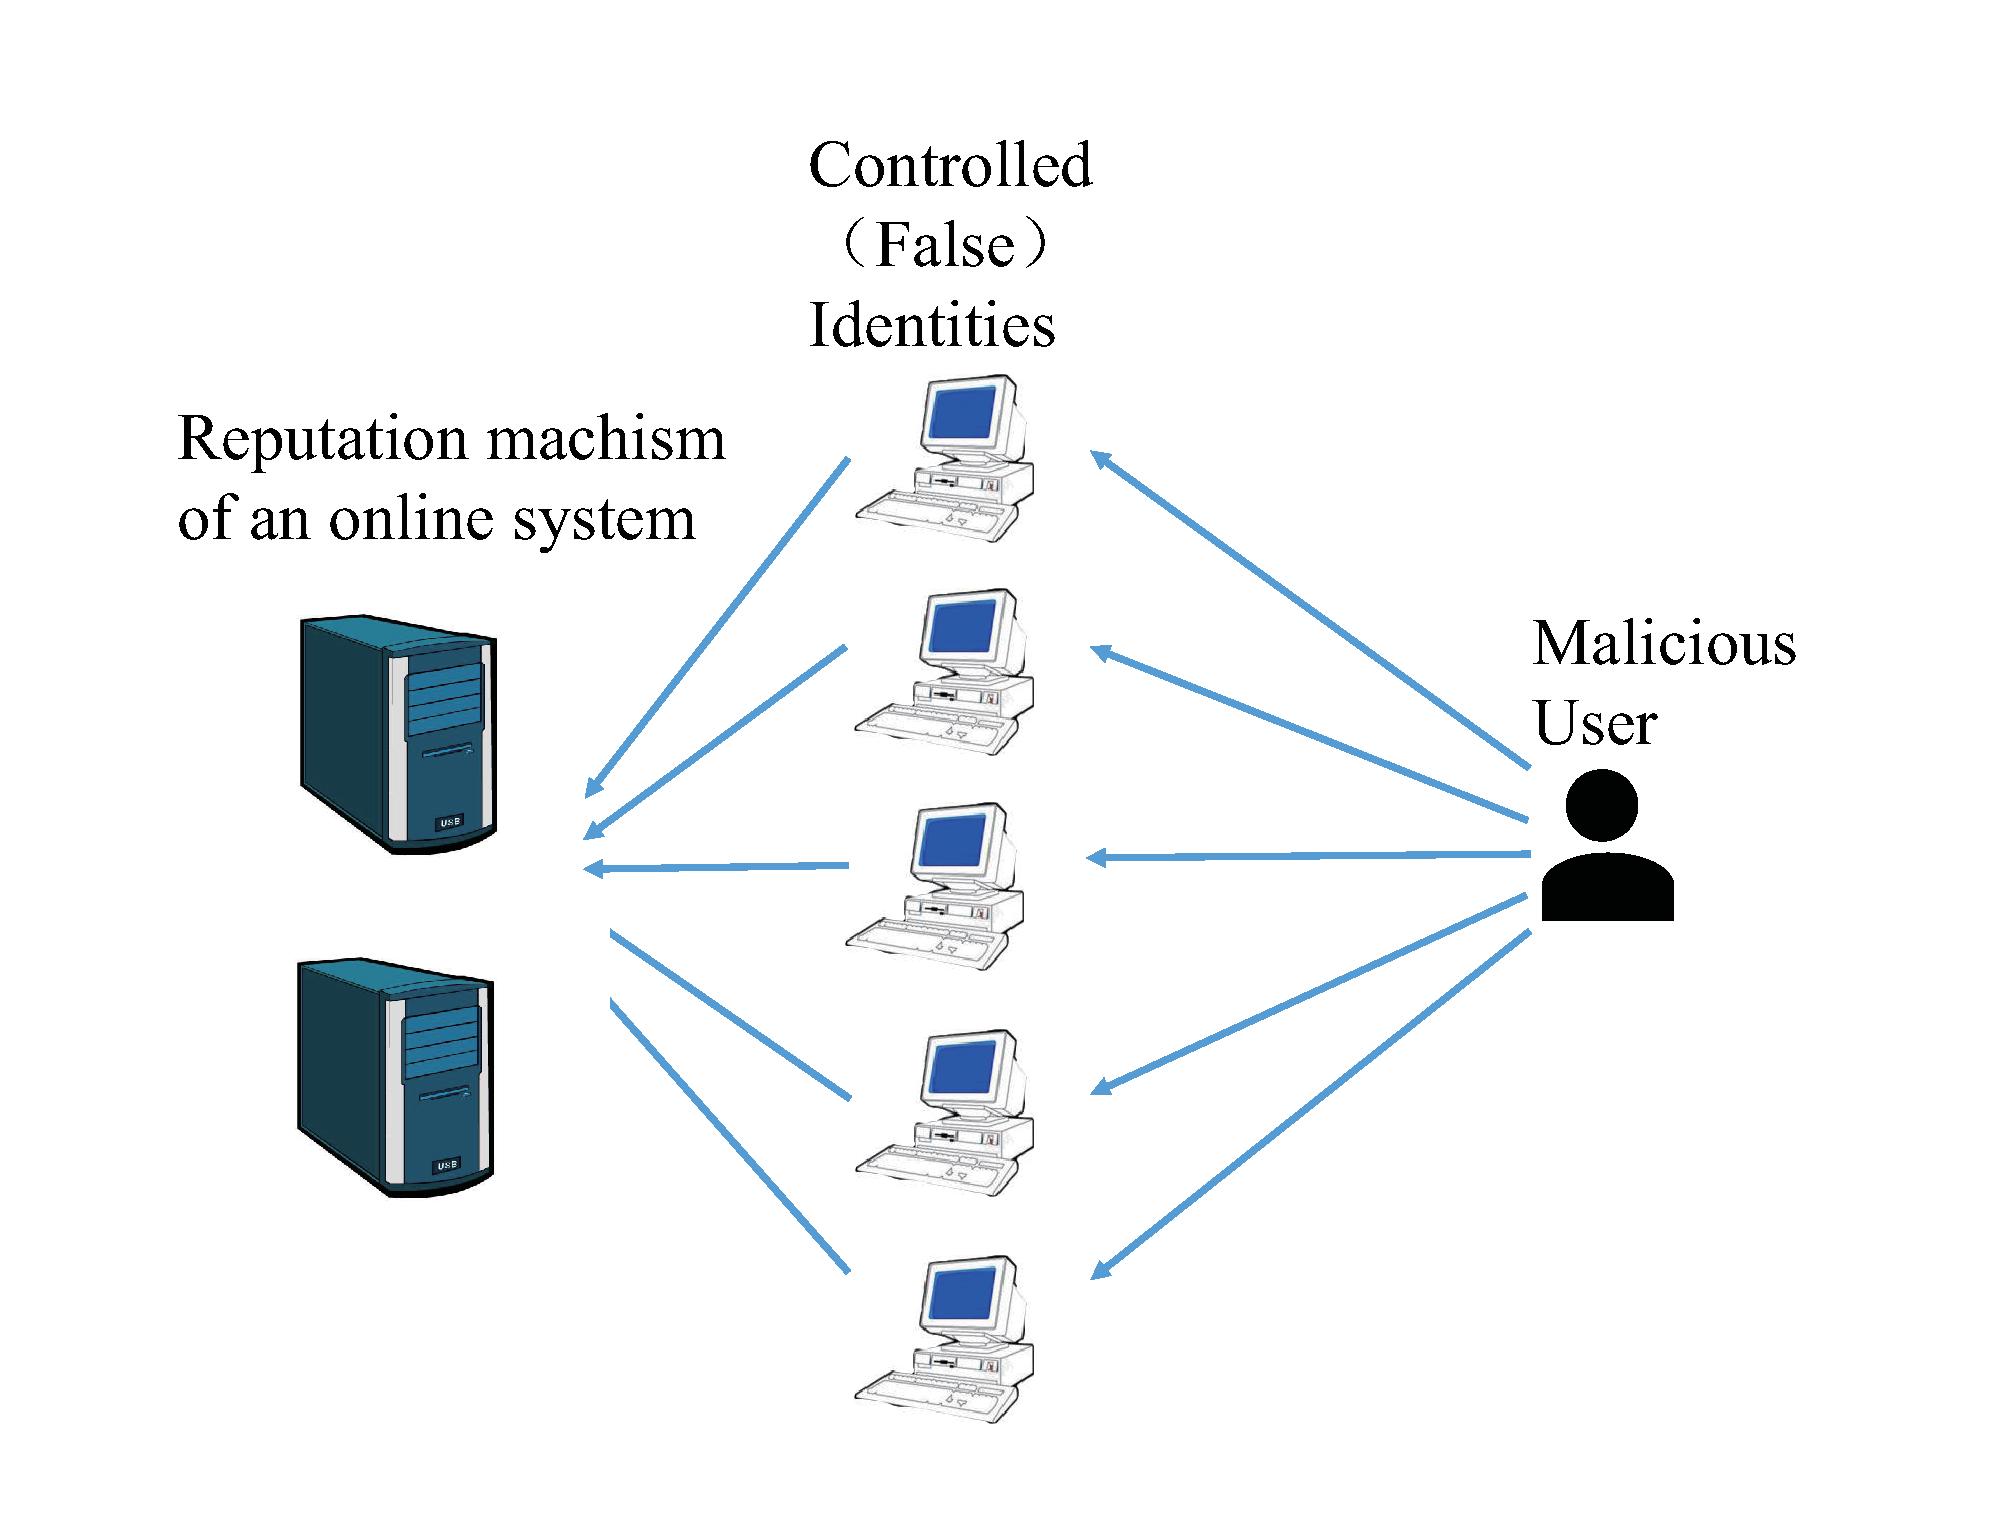
\includegraphics[width=1.0\linewidth,height=2.5in]{output/fig14.eps}
     \caption{The schematic of the Sybil attack. Malicious users create a
     large number of fake nodes and control them to disrupt the normal
     operation of the network.}
     \label{fig14}
\end{figure}

The first type of Byzantine attacks is the Sybil attack.
It was first proposed by John Douceur et al. in 2002~\cite{douceur2002sybil}
. As shown in Fig.~\ref{fig14}, it is a type of network security
attack where the attacker creates multiple fake identities
or nodes to undermine the network's trust mechanism and
disrupt its normal operation. The principle behind this
attack is that the attacker creates a large number of fake
identities, nodes, or accounts that appear independent and
genuine to the network but are actually controlled by the
attacker. The attacker can use various means to create
these fake entities, including using forged IP addresses,
anonymous proxy servers, virtual machines, and more.
This attack mainly targets systems that rely on trust
and identity verification mechanisms, such as
peer-to-peer networks, social networks, and blockchains. Attackers
can use a large number of fake identities to control the
resources of the system, deceive other users, and disrupt
consensus mechanisms. For example, in a peer-to-peer
network, attackers can create numerous fake nodes to
control the distribution process of files, leading to uneven
resource distribution or network performance degradation. 


The Sybil attack has posed significant threats to various
network security systems since it was proposed. Bhagoji
et al.~\cite{bhagoji2019analyzing}, Jun et al. ~\cite{lin2019free} and Yang et al.~\cite{yang2022overview} explore
it from the aspects of attack strategy, attack form and
attack field respectively. Bhagoji et al.~\cite{bhagoji2019analyzing} explore some
attack strategies against deep neural networks by
enhancing malicious agent updates and employing alternating
minimization strategies for stealth and adversarial targets.
They demonstrate the possibility of effective and covert
model poisoning attacks. Jun et al.~\cite{lin2019free} are the first
to explore the Freerider attack in federated learning and
propose an incremental weight attack method that can
evade most defense monitoring methods at that time. They
also introduce a new high-dimensional anomaly detection
method called STD-DAGMM, which is particularly useful
for detecting freeriders. This method has potential
applications for detecting other models' weight anomalies as well,
which will be discussed in the next chapter. Yang et al.~\cite{yang2022overview}
focus on the problem of vehicular ad hoc networks
and criticized previous studies for only considering the
security threats and impacts of Sybil attacks in VANETs
without analyzing the potential threats and impacts in
VFCs (Vehicular Fog Computing). Therefore, the authors
summarize four types of Sybil attacks that could affect
VFCs in areas such as routing, vehicle decision-making,
voting, and reputation systems. 

In recent years, Sybil attacks have undergone significant
development. Attackers employ more advanced techniques
to create false identities, making Sybil nodes more realistic
and difficult to distinguish. For instance, they may use
virtualization technology to create multiple independent
virtual machines, each with its own IP address and
network identifier. Attackers can also utilize social
engineering tactics and information acquisition methods to disguise
themselves as genuine users or obtain additional fake
identities through the authorization of legitimate users.
Furthermore, attackers might construct more complex and
realistic Sybil networks by leveraging shared information
in social networks. With the widespread use of mobile
devices and the wireless networks, Sybil attacks have also
started to increase in these environments. Attackers can
threaten the security of location services, social networks,
and mobile applications by utilizing false identities and
location information on mobile devices. In the future, Sybil
attacks can be more extensively applied to blockchain
technology, which enable attackers to manipulate
consensus algorithms, launch double-spending attacks, or
undermine the fairness of blockchain networks by controlling a
large number of counterfeit identities.  

\subsection{Transmission Process Attack}  
The second type of Byzantine attacks is based on
the transmission process. Byzantine attacks can occur
during the communication process between participants. Attackers can tamper with, delete, or insert malicious
messages to disrupt the transmission of model updates. 

Zhang et al.~\cite{zhang2015byzantine} propose a centralized related
probability small-scale attack (CDPS), which utilizes additional
information. For instance, fusion rules in fault diagnosis~\cite{kailkhura2013distributed}
 can be considered as existing knowledge usable
for optimizing attack tactics. One form of CDPS attack
involves collaborative efforts among malicious users who
engage in communication. Moreover, sharing of
information can assist malicious users in devising efficient attack
strategies. Generally, colluding malicious users~\cite{fatemieh2010secure,qin2013defending} 
first exchange measurement values to ensure more accurate
decisions on the licensed channel state and then report
the coordinated forged results to enhance attack power.
Moreover, Fatemieh et al.~\cite{fatemieh2011using} introduce another attack
model called the full-knowledge attack.  

Cooperative spectrum sensing (CSS) is considered a
promising method for identifying available spectrum.
However, it not only requires a significant amount of
communication resources but also introduces vulnerabilities to
Byzantine attacks. Wu et al.~\cite{wu2018sequential} mention that attackers
keep reporting false information to the fusion center
consistently. In fact, attackers may attack discontinuously
while appearing normal during rest periods. The authors
propose a low-complexity sequential 0/1 (S0/1) method
for CSS in the presence of strategic Byzantine attacks.
It does not require strong assumptions or any prior
knowledge, and this method will be discussed in the next
chapter.

With the development of IoT devices, attackers may
exploit communication vulnerabilities and weaknesses
between IoT devices to launch future attacks. Attackers may
also utilize high-speed, low-latency 5G/6G networks to
carry out large-scale distributed denial-of-service (DDoS)
attacks, bypass security measures using network slicing
and virtualization technologies, or exploit vulnerabilities
in mobile communication protocols to attack devices and
systems.  

\subsection{Model Aggregation Attack}  
The third type of Byzantine attacks is known as model
aggregation attack. In this type of attack, Byzantine
attackers manipulate the model parameters of the
participants in order to influence the aggregation results.  

\begin{figure}[h]
    \centering
    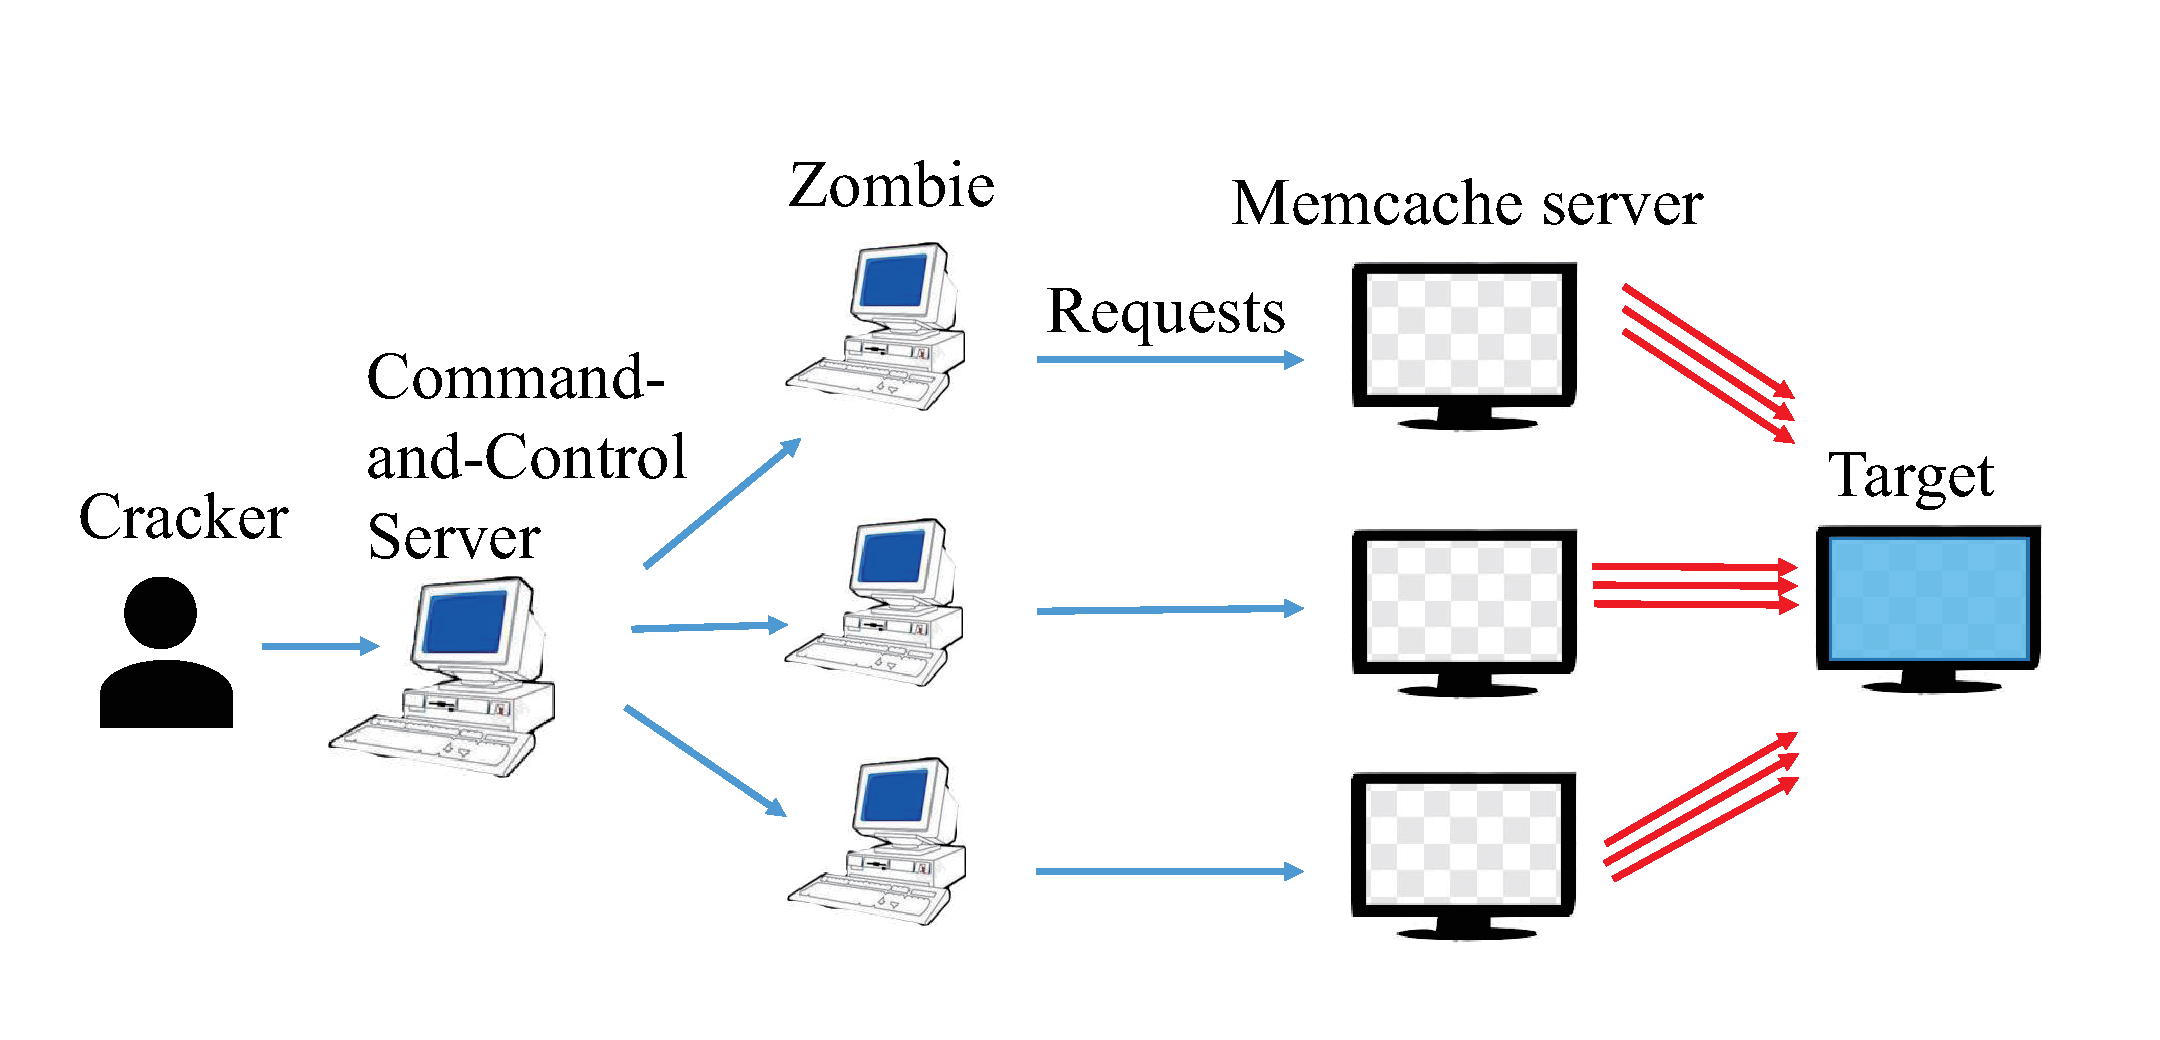
\includegraphics[width=1.0\linewidth,height=2.5in]{output/fig15.eps}
     \caption{The schematic of a DDOS attack. Through the central
     control system, the attacker uses specific software or malicious code
     to remotely control multiple zombies, making them send a large
     number of requests to the target system at the same time to exhaust
     the processing power, network bandwidth or resources of the target
     system, thus causing the target system to fail to work normally.}
     \label{fig15}
\end{figure}

As discussed by El Mhamdi et al.~\cite{guerraoui2018hidden}, these attacks by
Byzantine workers may not prevent the model from
converging but can instead lead to convergence on suboptimal
solutions. This is a new way of thinking and there is a lot of
room for development in the future. However, most attacks
disrupt the convergence of the model. Xie et al.~\cite{xie2018generalized}
propose a form of attack called Gamber. In this attack,
an attacker can modify some of the data communicated
between participants. The attacker randomly selects data
and makes malicious changes to them. The authors also
mention several other attacks,such as omniscient. The
attacker needs to have knowledge of the gradients sent by
all the staff members and replaces some gradient vectors
by taking the sum of all gradients, scaled by large negative
values. The objective is to mislead the Stochastic Gradient
Descent (SGD) algorithm into moving in the opposite
direction with larger step sizes. Weaker attacks, such as
Gaussian attacks, are also possible.In these attacks, some
gradient vectors are replaced with random vectors sampled
from a Gaussian distribution that has a large variance.
Such attackers do not require any information from the
staff members.  

\begin{figure}[h]
    \centering
    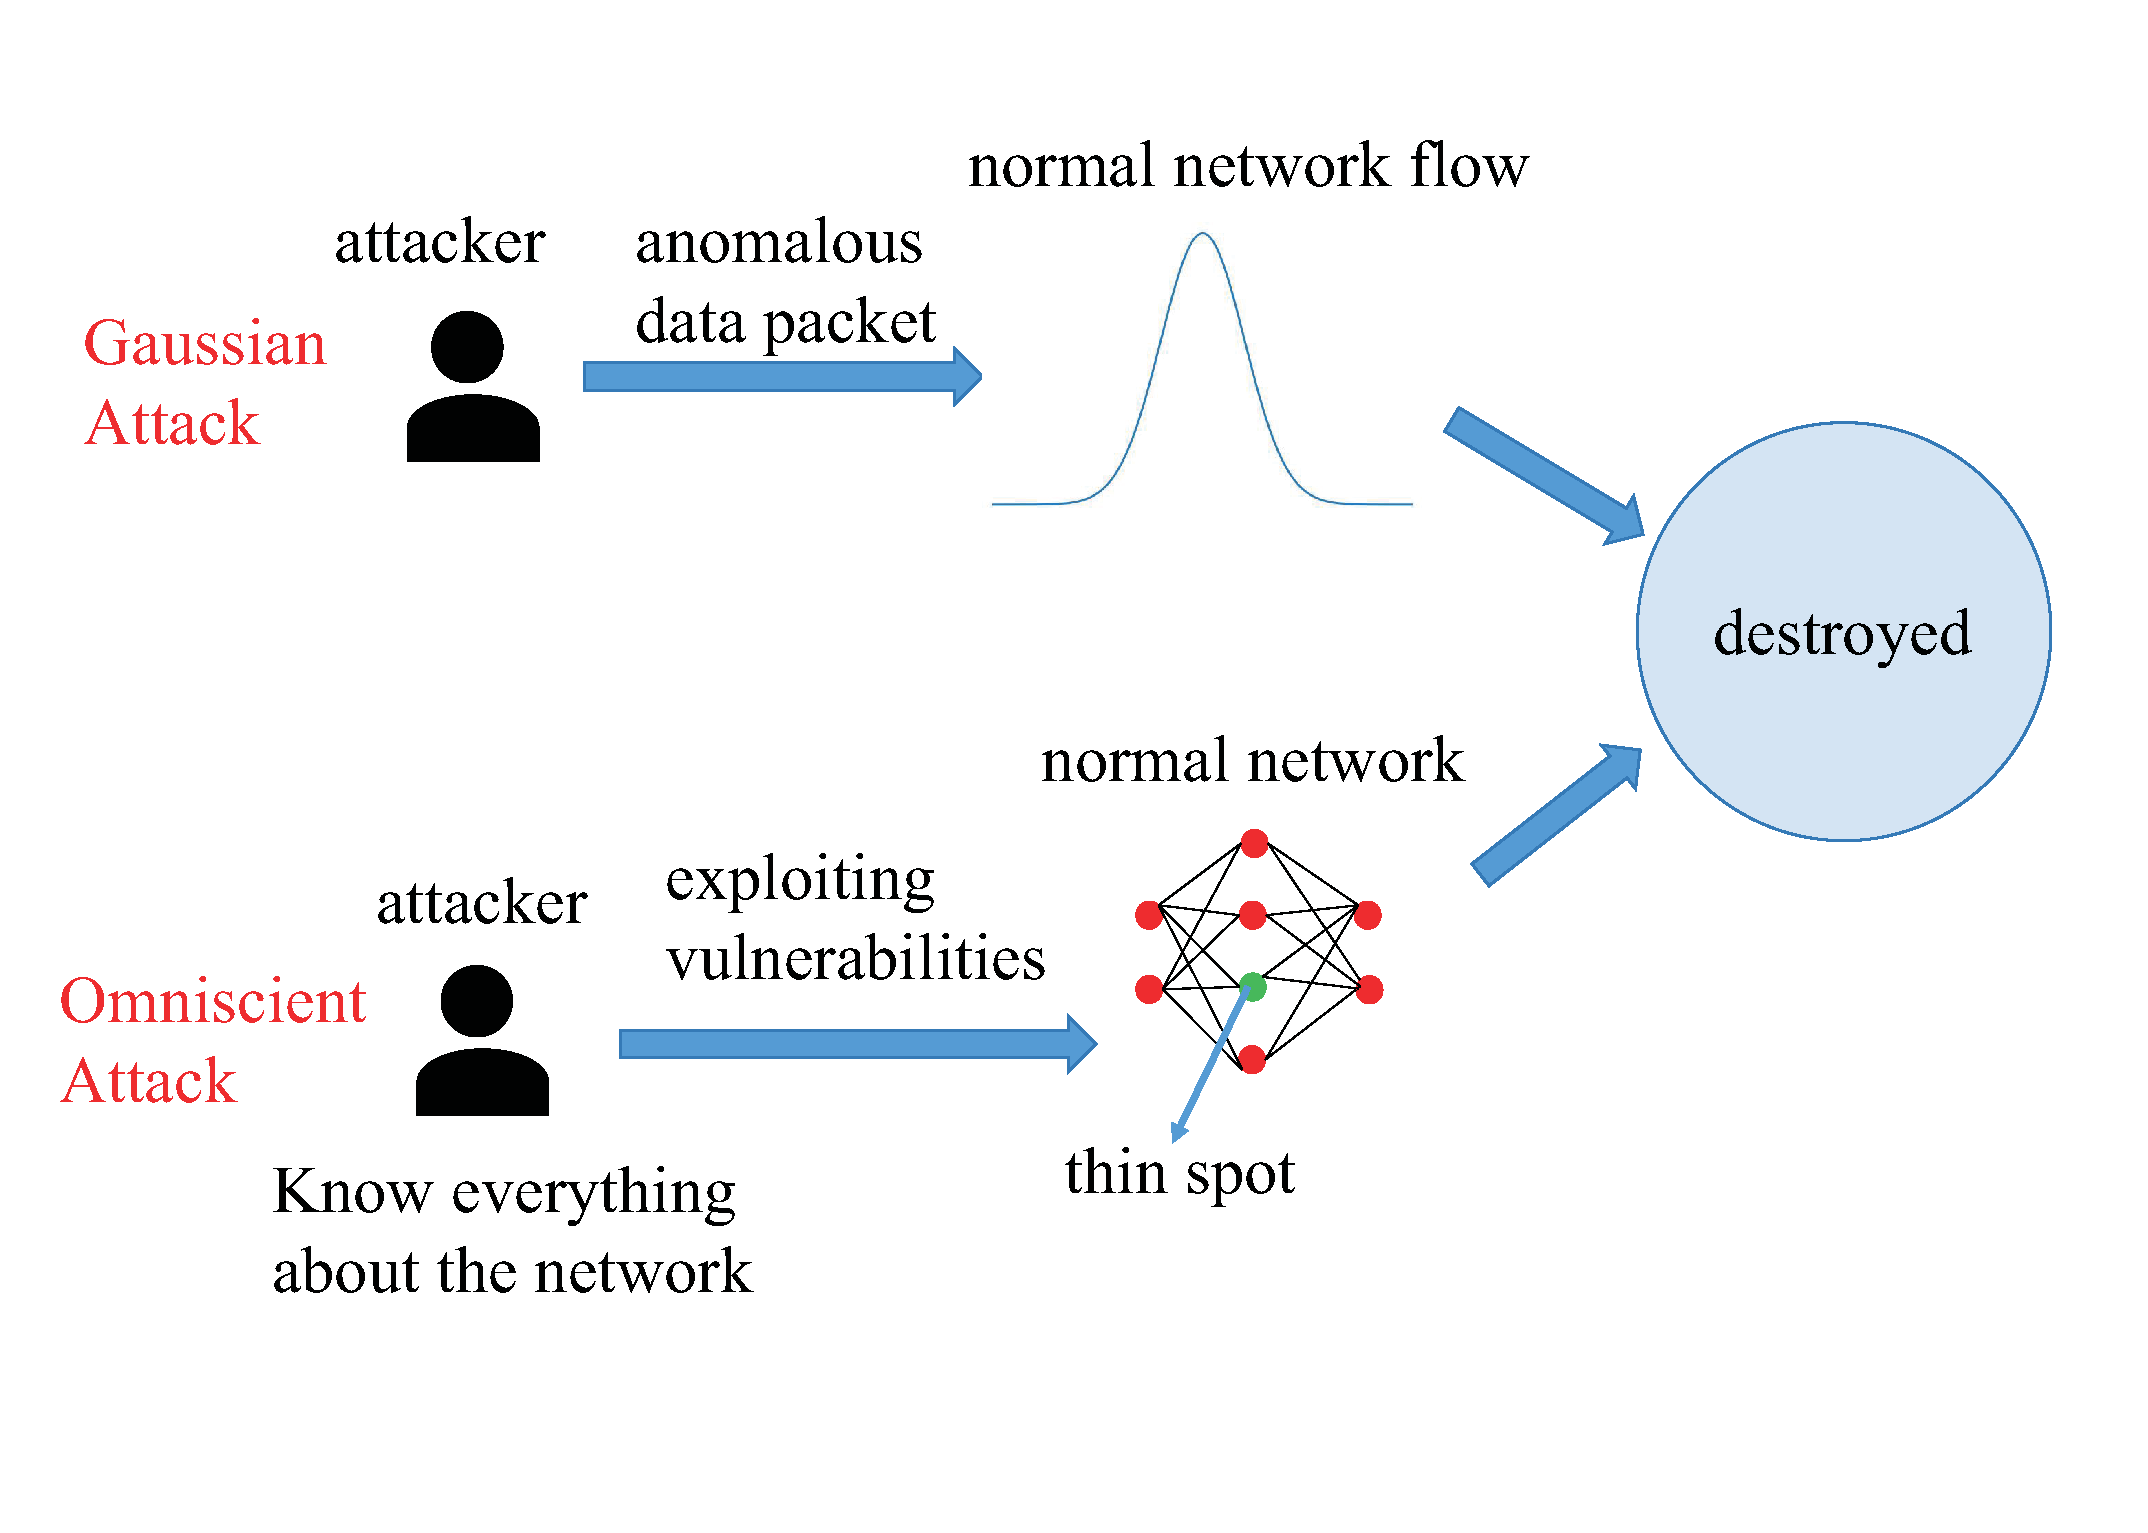
\includegraphics[width=1.0\linewidth,height=2.5in]{output/fig16.eps}
     \caption{The schematic of Gaussian attack and Omniscient attack.In
     a Gauss attack, an attacker enters incorrect packets into the network,
     affecting the normal running of network flows.An omniscient attack is
     a hypothetical scenario where an adversary has complete and perfect
     knowledge or awareness of the system they are targeting. In this
     type of attack, the adversary has access to all the information and
     capabilities necessary to exploit vulnerabilities in the system. With
     this all-encompassing knowledge, the attacker can strategically plan
     and execute attacks to maximally exploit the system’s weaknesses.}
     \label{fig16}
\end{figure}


In many applications, multiple sources can provide
descriptions of the same object or event, which can inevitably
lead to conflicts in data or information. Resolving conflicts
in data is an important challenge in achieving convergence
in federated learning. Byzantine attackers have the ability
to exploit these issues in order to manipulate the
convergence of the model. Li et al.~\cite{li2014resolving}, Hsu et al.~\cite{hsu2019measuring}, and
Jiang et al.~\cite{jiang2023secure} have all explored questions related to
data differences and conflicts. 

In future attacks, attackers may attempt to achieve their
objectives by making modifications to the trained model.
This can involve incorporating backdoors into the model,
which would produce incorrect outputs under specific
conditions, or tampering with the model parameters to
disrupt its robustness. In order to evade detection, future
attack strategies could involve the development of more
advanced and covert techniques to camouflage malicious
modifications. Additionally, malicious insiders who have
access to the model parameters may exploit this privilege
to launch attacks. They could manipulate the parameters
to compromise the model's performance or even insert
sensitive information within the model itself. In the coming
years, attackers may explore more complicated techniques
and algorithms to bypass security monitoring and
detection mechanisms. The aim would be to implement internal
personnel attacks more efficiently. These advancements
would allow attackers to bypass existing safeguards and
carry out their malicious activities with greater precision
and effectiveness.  

\section{Defenses Against Byzantine Attack}  
With the advancement of Byzantine attacks, the
corresponding defense methods are constantly evolving and
being updated. As shown in Fig.~\ref{fig12}, based on the different
types of Byzantine attacks discussed in the previous
chapter, we categorize the Byzantine defense methods into
three classes:  

\subsection{Defenses against Sybil Attack}  
For Sybil attacks, the defense methods include trust-based
evaluation methods and machine learning models
for detecting fake nodes. Gil et al.~\cite{gil2017guaranteeing} propose a novel
algorithm that analyzes received wireless signals to detect
the presence of deceptive clients created by adversaries.
It does not require specialized hardware or private key
exchanges, commercial Wi-Fi cards and software are
enough. It utilizes the physical characteristics of wireless
signals to ”perceive” deceivers. The authors conduct
experiments using the AscTec quadcopter server team and
iRobot Create ground clients, which show a deception
detection rate exceeding 96Blanchard et al.~\cite{blanchard2017machine} introduce
Krum, which detects and removes outliers in gradient
aggregation, allowing convergence even in the presence
of multiple Byzantine attackers, and with low complexity.
Gil et al.~\cite{gil2017guaranteeing} and Blanchard et al.~\cite{blanchard2017machine} reduce the impact
of the attacker, but don't accurately detect the attacker
and remove it.  

\begin{figure}[h]
    \centering
    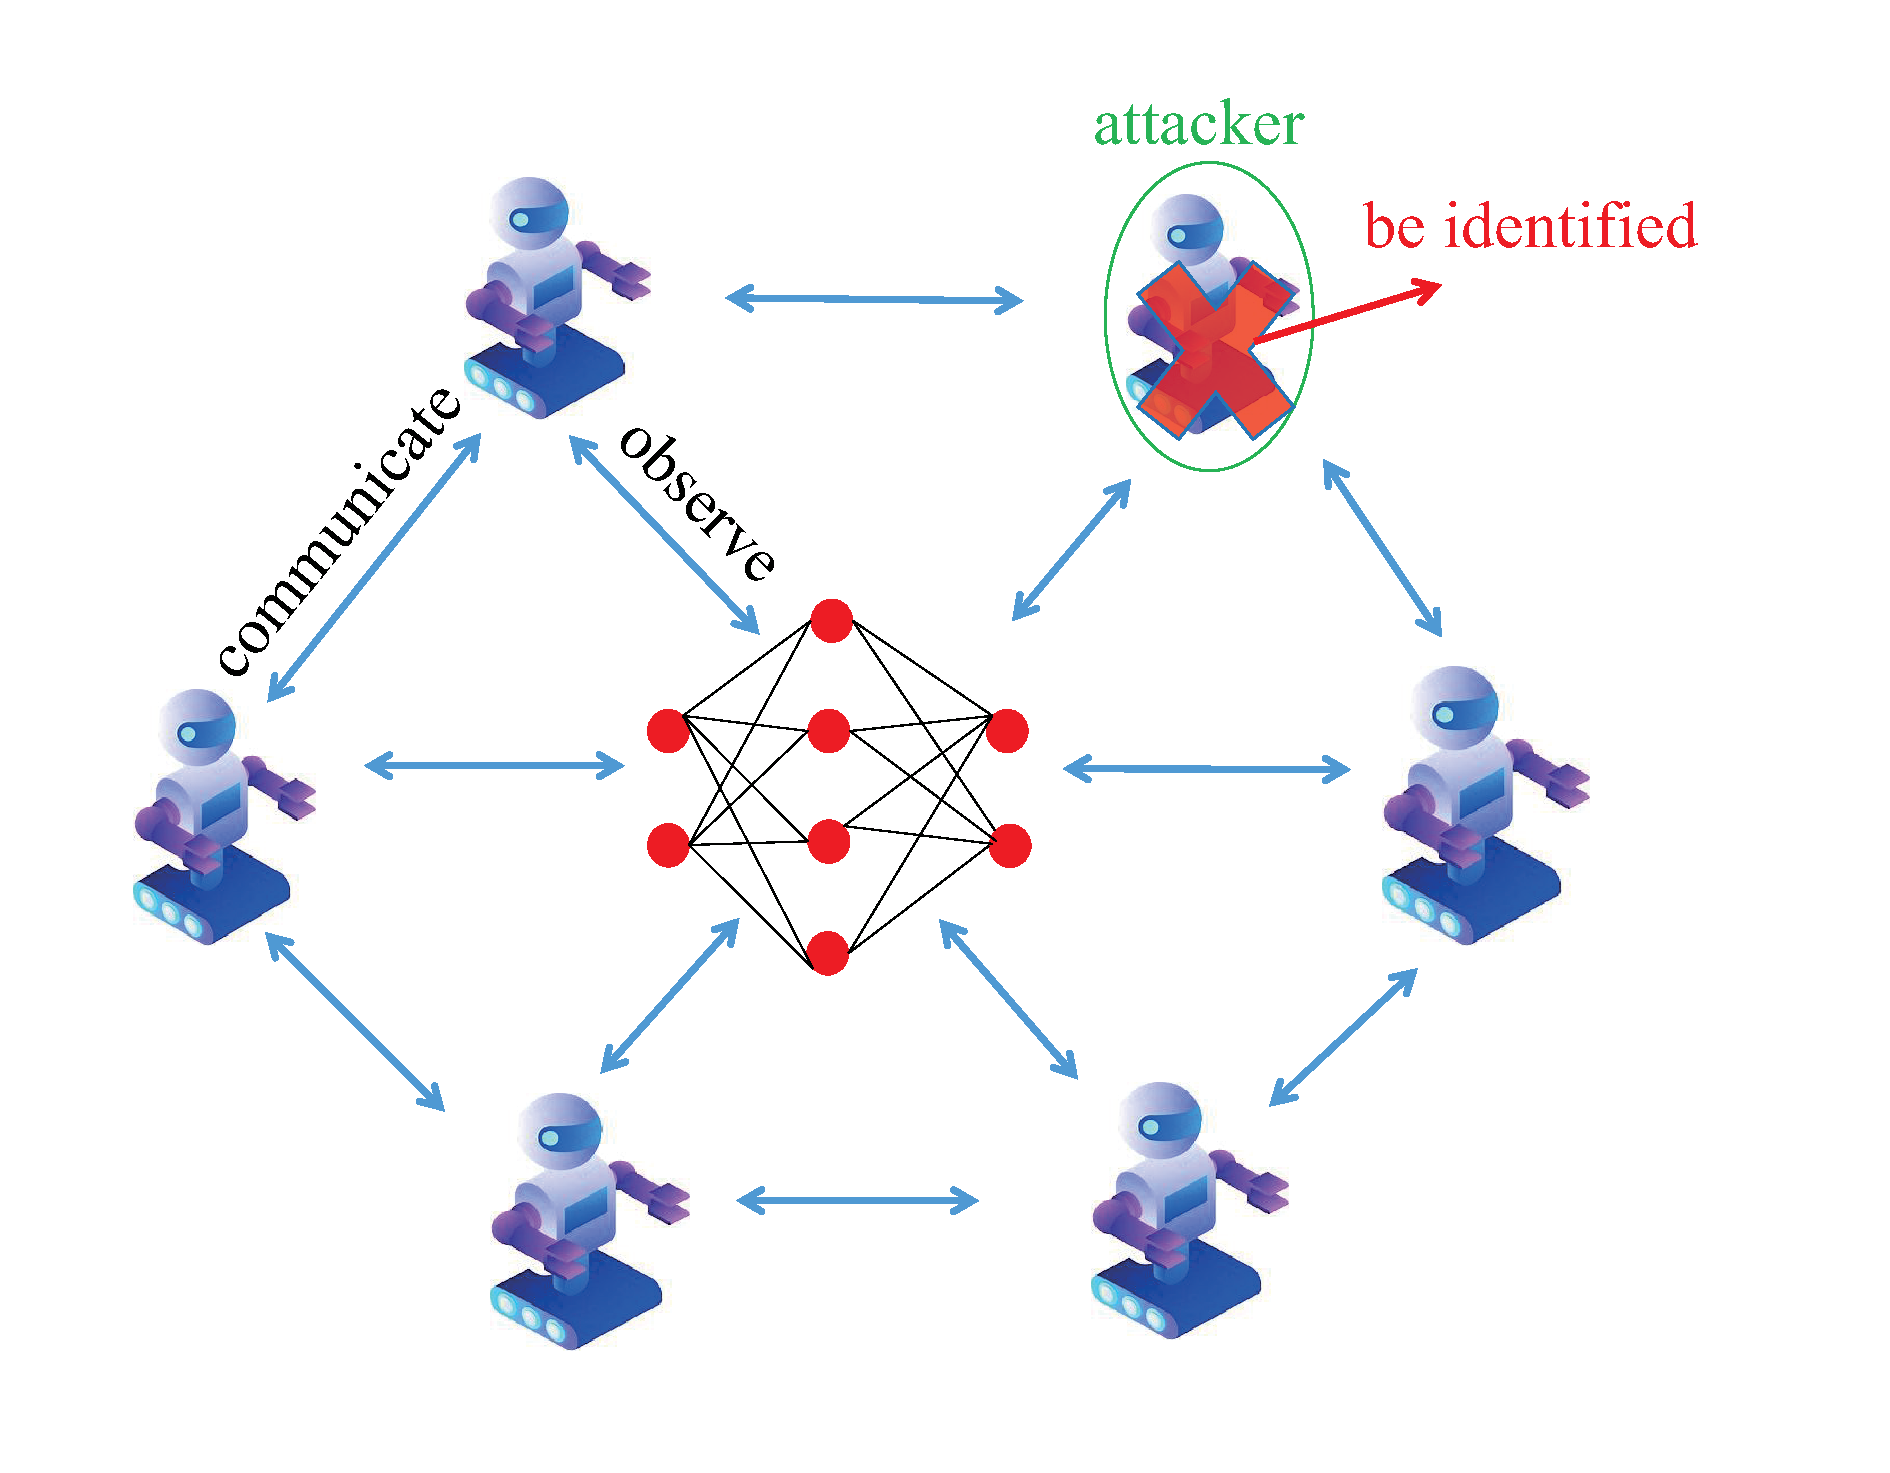
\includegraphics[width=1.0\linewidth,height=2.5in]{output/fig17.eps}
     \caption{Robots can communicate with neighbors to get information,
     combined with their own information, in a certain round can
     eliminate the interference of malicious robots, reach a consensus.}
     \label{fig17}
\end{figure}


Both of the following methods detect the malicious
attacker and remove its effects. Muñoz-González et al.~\cite{munoz2019byzantine}
 propose a new algorithm for robust federated learning
called Adaptive Federated Averaging, aims to detect
faults, attacks, and malicious updates provided by
participants in a collaborative model. The authors also propose
a Hidden Markov model to simulate and learn the quality
of model updates provided by each participant during
training. In the work of Mallmann-Trenn et al.~\cite{mallmann2021crowd}, a
combination of wireless signal analysis and observations
from sociological learning is used to demonstrate rapid
convergence of correct trust values for all robots in the
team when facing attacks. All robots develop their own
opinions about network trust by observing messages sent
through the network as shown in Fig.~\ref{fig17}. They compare
their opinions with those of their neighbors to reach
a consensus on whether the robots can be trusted. By
utilizing their neighbors' opinions, each robot effectively
increases the number of observations available to them
about the network, thereby eliminating messages with a
high probability of coming from malicious robots through
cross-validation. Experiments show that in a limited
number of communication rounds, all robots agree on the
global consensus of trustworthiness in their neighborhood. 

Sybil attacks pose a significant challenge as attackers
can create a large number of false identities, making it
difficult to detect and differentiate them. Therefore,
developing secure systems requires consideration of multiple
defense methods and selecting appropriate solutions based
on specific application contexts. The future outlook for
such defense techniques primarily focuses on the following
areas: enhancing identity verification mechanisms to
distinguish genuine users from Sybil nodes and establishing
stronger trust mechanisms to identify and filter out Sybil
nodes displaying malicious behavior. In recent years,
the emergence of blockchain technology has provided a
decentralized, tamper-resistant, and secure shared ledger,
offering a potential defense against Sybil attacks. By
combining identity verification, trust mechanisms, and
blockchain technology, the ability to detect and prevent
Sybil nodes can be improved.  

\subsection{Defense Against Transmission Process Attack}  
Defense methods against attacks during the transmission
process include designing secure communication
protocols and encryption mechanisms. Previous malicious detection and suppression
algorithms focused only on simple ”always attack” scenarios,
where attackers continuously report false information to
the central entity. In reality, attackers may intermittently
attack while behaving normally at other times. Under the
assumption of simple attack strategies, Chen et al.~\cite{chen2012robustness}
propose sequential hypothesis testing to defend against
Byzantine attacks, but it requires significant
computation and prior knowledge. Therefore, Wu et al.~\cite{wu2018sequential}
introduce S0/1 using support vector regression (SVR)
to offset strategic Byzantine attack defense. Even in a
blind scenario, this approach greatly reduces the sample
size while providing higher correct sensing ratios.
MuñozGonzález et al.~\cite{munoz2019byzantine} also propose a robust aggregation
rule that detects and discards malicious or poor local
model updates during each training iteration. It includes
mechanisms for blocking unwanted participants, thereby
enhancing computational and communication efficiency.  

In traditional federated learning, the performance of
models may decline due to variations in data distributions
across devices. To solve this problem, Mostafa et al.~\cite{mostafa2019robust}
propose a technique called ”representation matching.”
This technique improves model performance by matching
features between the global model and local models. For
clients with homogeneous data distributions, this approach
consistently improves accuracy. For heterogeneous clients,
in addition to improving accuracy, this approach enhances
training robustness and avoids catastrophic training
failures without the need for manual hyperparameter tuning
for each task.  

\begin{figure}[h]
    \centering
    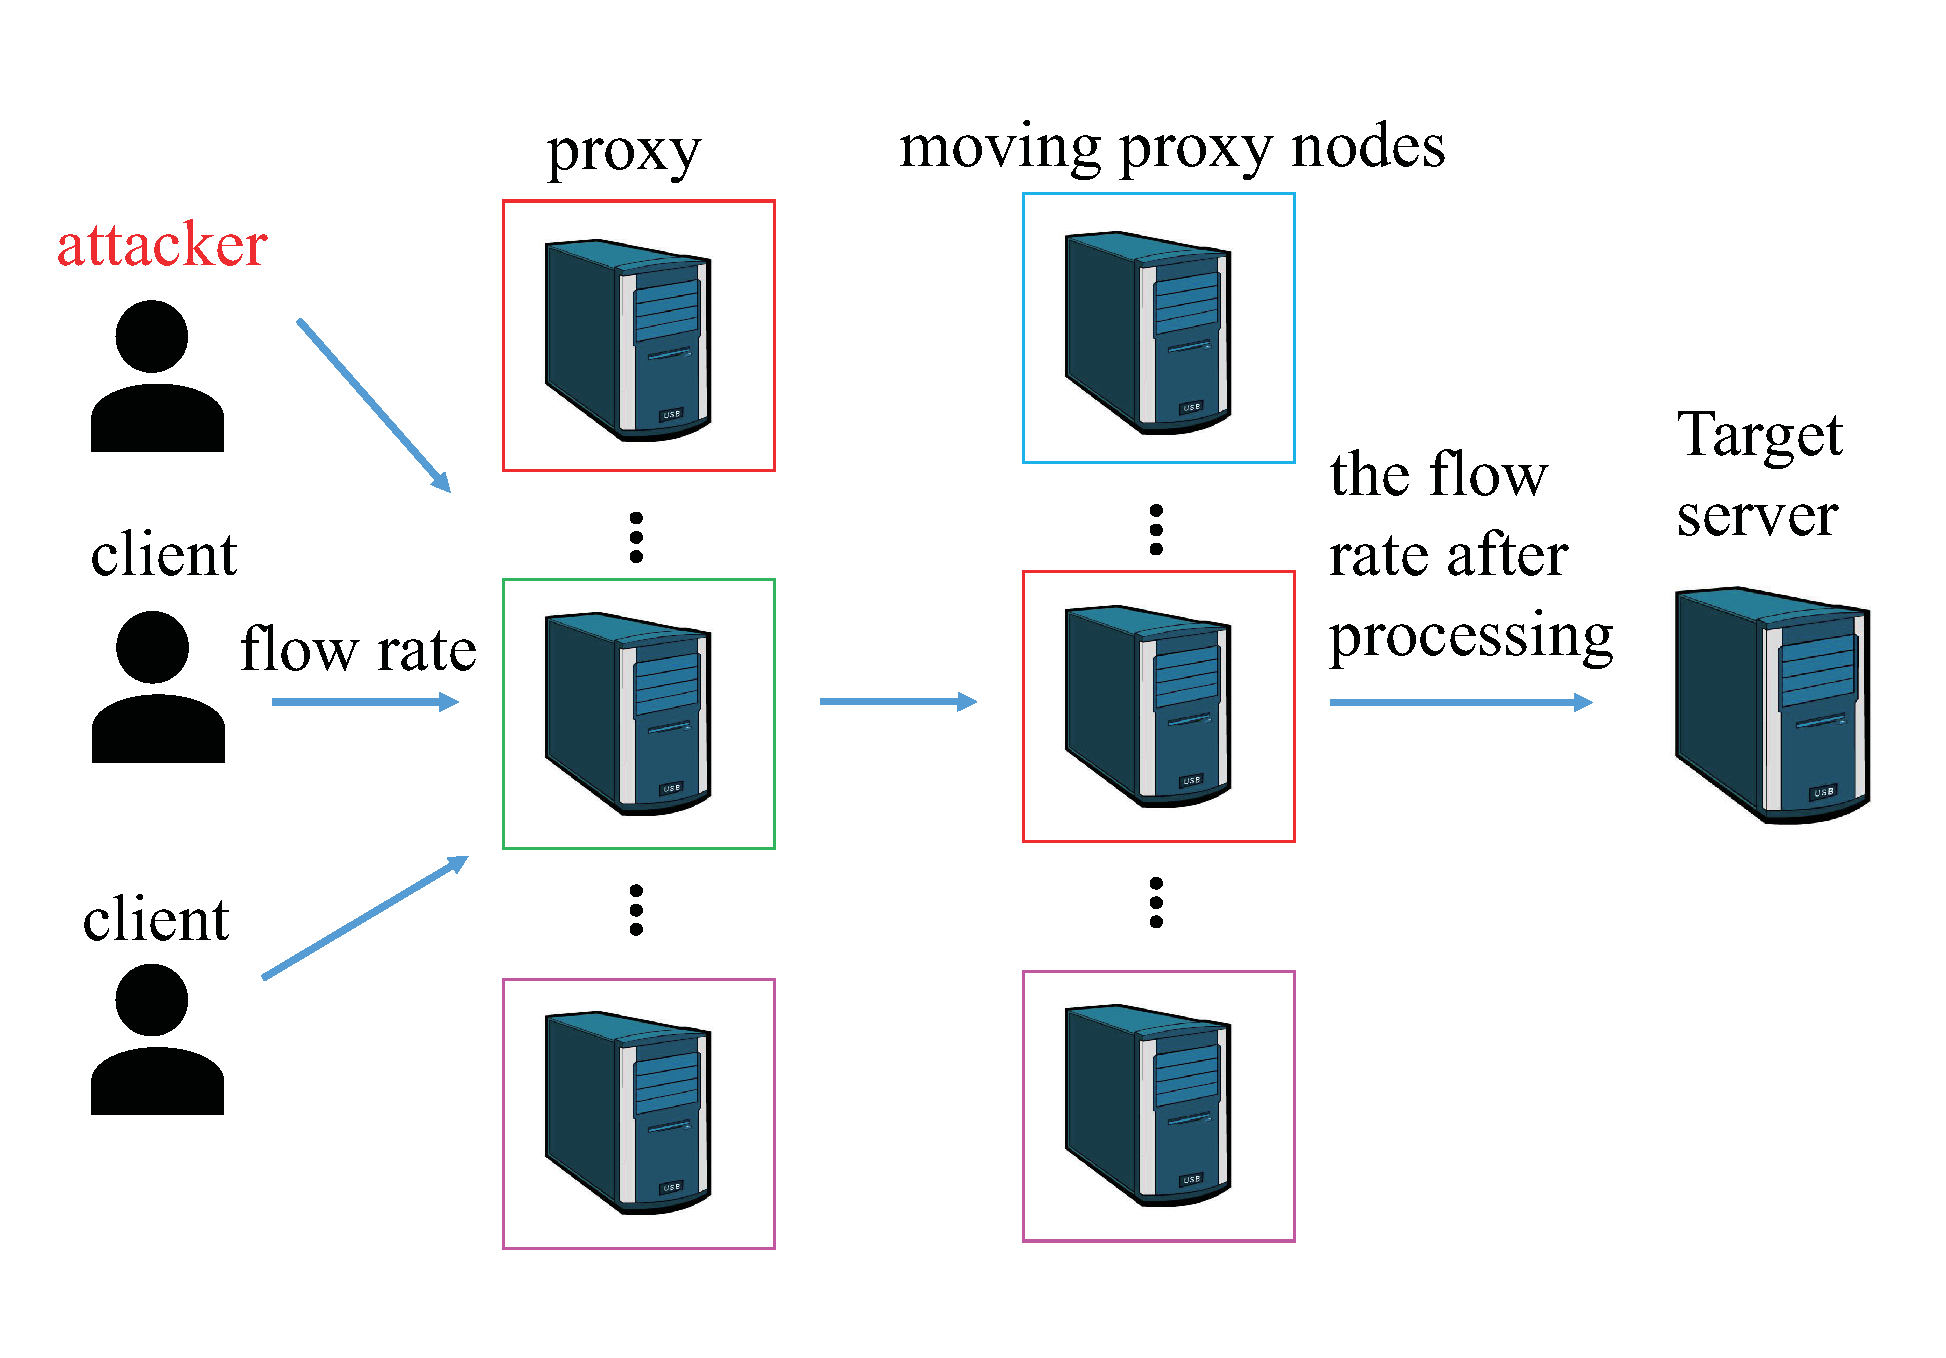
\includegraphics[width=1.0\linewidth,height=2.5in]{output/fig18.eps}
     \caption{DDOS defense method of secret moving proxy nodes.The
     proxy node is constantly moving its position, confusing the attacker
     so that it cannot find the real target server.}
     \label{fig18}
\end{figure}


Wang et al.~\cite{wang2014moving} propose a mobile target defense mechanism that specifically
addresses DDoS attacks targeting authenticated clients of Internet services.
This mechanism utilizes a set of dynamic and hidden proxies to relay traffic
between authenticated clients and servers. As shown in Fig.~\ref{fig18}, by continuously
replacing the attacked proxies with backup proxies and reallocating attacked
clients to new proxies, innocent clients are separated from malicious insiders
through a series of shuffling. In recent years, significant efforts have been
made to defend against lowrate DDoS attacks. Attackers easily launch complex
lowrate DDoS attacks by exploiting prominent features of cloud computing.
Therefore, research on various DDoS attacks and their corresponding defense
methods is crucial in protecting cloud infrastructure from devastating impacts
of DDoS attacks. Agrawal et al.~\cite{agrawal2019defense} conduct a comprehensive classification of
all possible variants of cloud DDoS attack solutions and provide detailed
insights into characterization, prevention, detection, and mitigation mechanisms.

In the future, these defense methods can be further
developed by constructing more secure and robust
encryption protocols and algorithms. Additionally, more effective
Identity verification technologies can be developed to
ensure the trustworthiness of communication parties.
Continual improvement and enhancement of transport layer
protocols, such as SSL/TLS, can provide stronger security
and defense capabilities, including the ability to resist
man-in-the-middle attacks, data tampering, and replay
attacks. The development of real-time threat detection
systems capable of detecting and responding to attacks
during the transmission process can also be explored.With
the advancement of quantum computing, traditional
encryption algorithms may be threatened. Therefore,
researching and developing quantum-safe communication
protocols and algorithms is also important to ensure
security during the transmission process and protect data
confidentiality in a quantum computing environment. 

\subsection{Defense Against Model Aggregation Attack}  
Defense methods against model aggregation attacks
include designing robust aggregation algorithms and using
differential privacy techniques to protect model parameters.

El Mhamdi et al.~\cite{guerraoui2018hidden} argue that mere convergence of
the Byzantine resilient rules is not enough. It is possible
that Byzantine workers' attacks can lead to convergence
to the worst suboptimal solution. To address this, they
propose a generic enhancement method called Bulyan.
This method significantly reduces the leeway for
Byzantine workers, constraining them within narrow boundaries.
For common batch sizes, Bulyan achieves performance
comparable to average speed. 

Li et al.~\cite{li2014resolving},Hsu et al.~\cite{hsu2019measuring} and Jiang et al.~\cite{jiang2023secure}
work on issues about data heterogeneity and conflicts.
Li et al.~\cite{li2014resolving} model the problem using an optimization
framework where ground truth and source reliability are
defined as two sets of unknown variables. The objective
is to minimize the overall weighted differences between
the ground truth and multiple-source observations, with
each source weighted by its reliability. This framework
can incorporate different loss functions to identify
features of various data types and has developed efficient
computing methods that effectively identify the true
information among conflicting data sources. Hsu et al.~\cite{hsu2019measuring}
 present a method for synthesizing datasets with
continuous identical ranges and provide performance
metrics for the federated averaging algorithm. Experimental
results demonstrate that performance deteriorates with
distribution differences. The proposed method suppresses
oscillations through the accumulation of gradient history,
and it has been shown that using momentum on top
of SGD for non-iid problems has achieved significant
success in accelerating network training. Jiang et al.~\cite{jiang2023secure}
introduce the combination of handling imbalanced data
and Byzantine attacks in the context of federated learning
for the first time. The concept of an intelligence pool is
proposed to separate the task of judging the shared local
model values from the aggregator, avoiding the limitations
of a single criterion through two-layer verification shown
in Fig.~\ref{fig19}.

Xie et al.~\cite{xie2018generalized},Portnoy et al.~\cite{portnoy2020towards} and Pillutla et
al.~\cite{pillutla2022robust} propose several rules or algorithms to make
the model aggregation work smoothly. Xie et al.~\cite{xie2018generalized}
introduce three robust aggregation rules for stochastic
gradient descent (SGD) with low computational costs.
These rules are the first to be theoretically and empirically
studied under the non-convex setting, based on median
aggregation. Portnoy et al.~\cite{portnoy2020towards} propose a novel method
called Byzantine Robust Client Weighting (BRCW) to
minimize the impact of malicious clients in federated
learning. BRCW assigns different weights to each client
based on their credibility and contribution to the overall
model accuracy. During training, the weights are
dynamically updated according to each client's performance
and behavior. Unlike previous work, this study considers
the sample size provided by clients as untrustworthy,
as it may come from malicious clients. BRCW exhibits
robustness against various forms of attacks, including
communication disruptions and data poisoning. Pillutla
et al.~\cite{pillutla2022robust} design a novel robust aggregation oracle based
on classical geometric medians and demonstrate its
robustness in federated learning with limited heterogeneity, even
when up to half of the devices are faulty. The proposed
RFA algorithm outperforms the standard FedAvg (14)
in high damage scenarios and nearly matches FedAvg's
performance in low damage scenarios, but with 1-3 times
higher communication costs. 

\begin{figure}[h]
    \centering
    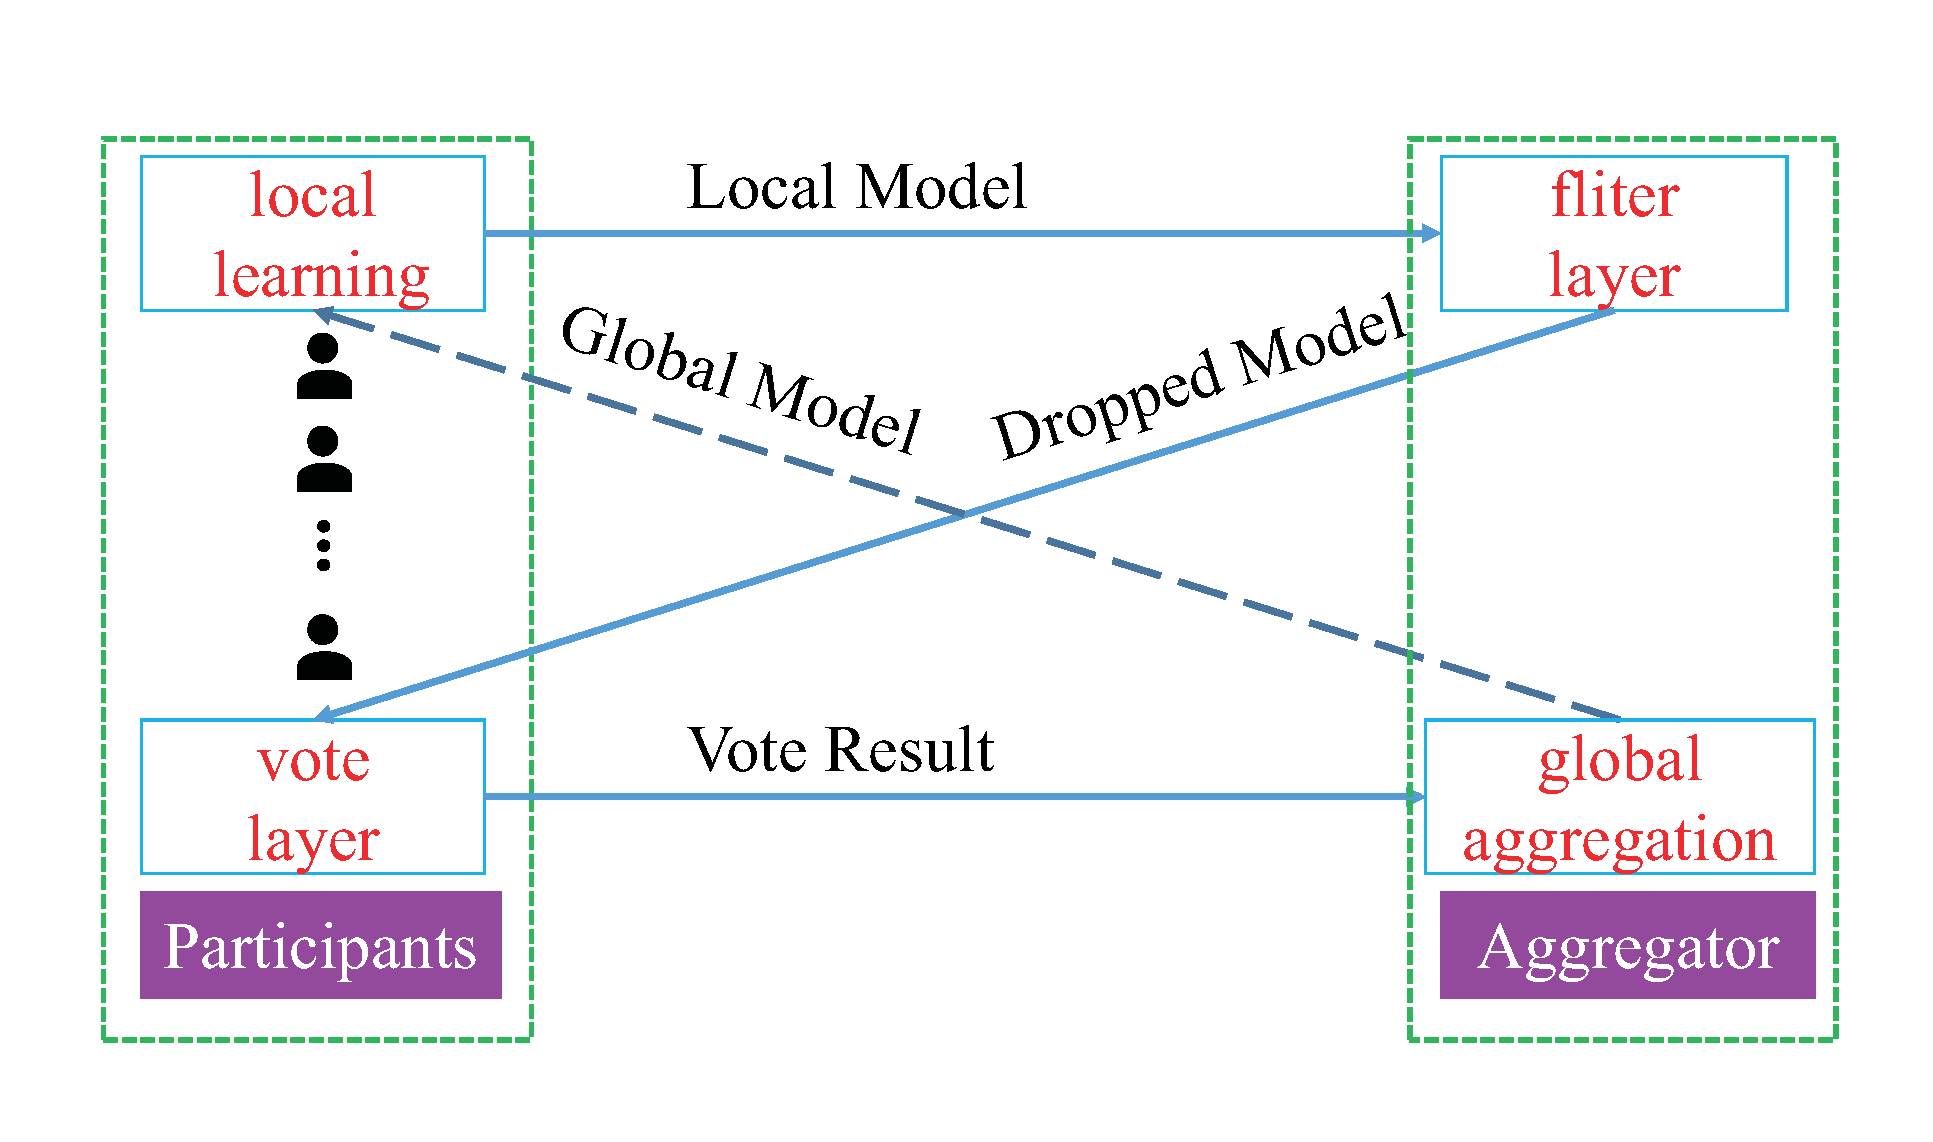
\includegraphics[width=1.0\linewidth,height=2.5in]{output/fig19.eps}
     \caption{The structure of two-layer aggregation method. Participants
     share the global model, and models discarded by the filter layer are
     not directly abandoned, but are voted by participants to participate
     in the final aggregation process.}
     \label{fig19}
\end{figure}


Future prospects for such defense methods will
focus on more stricter authentication and authorization
mechanisms, as well as parameter integrity protection.
Mechanisms such as Hash algorithms or digital signatures
can be adopted to safeguard the integrity of parameters,
preventing tampering during transmission and storage.
Detection of malicious parameter modifications and
corresponding response measures are also required.
By comprehensively applying these methods, the defense capability
against malicious parameter modification attacks can be
enhanced, ensuring the security and integrity of systems
and applications.